\documentclass[../main.tex]{subfiles}
\begin{document}
\section{Flujo de Información y Malware}

Esta unidad retoma el problema del flujo de información (ya visto informalmente
al hablar de políticas) y lo formaliza con la \textbf{entropía}. Cierra el bloque
de seguridad en aplicaciones y luego cambia de perspectiva (la del atacante) para
introducir el \textbf{malware}. Lectura recomendada: Bishop, \textit{Computer
Security: Art and Science}, capítulos 16 (parte 1) y 17.

%======================================================================
\subsection{Flujo de información: el problema}
%======================================================================

Las políticas de seguridad rara vez se expresan como permisos sobre objetos. Una
política típica dice: \emph{``un empleado no puede ver los sueldos de otros
empleados''}. El profesor remarca que ese requisito se refiere a \textbf{la
información en sí}, no al lugar donde la información está en un momento puntual.

\begin{definicion}{Control de acceso vs.\ control de flujo}
\textbf{Control de acceso:} limita el acceso de un \emph{sujeto} a una
\emph{operación} puntual sobre un \emph{objeto} puntual. Como los objetos
contienen información, indirectamente limita el acceso a información.

\textbf{Control de flujo:} estudia cómo la información \emph{se mueve} a través
del sistema. La información no es estática: \textbf{se actualiza y se puede copiar}.
\end{definicion}

El control de acceso \textbf{no impide copiar la información a otro lugar}: un
usuario con permiso de lectura sobre su sueldo puede leerlo y escribirlo en un
objeto que otros puedan ver (camino de lecturas y escrituras).

\begin{destacado}
Las políticas \textbf{por lo general restringen el flujo de información y no el
acceso a objetos}. Comparar: ``evitar que un empleado sepa el sueldo de otro''
(flujo) vs.\ ``evitar que un empleado acceda a la base de datos de sueldos''
(acceso). El control de acceso \emph{sirve}, pero son \textbf{mecanismos abiertos}:
aseguran una parte del problema, no todo. Deben ser \textbf{complementados}.
\end{destacado}

\begin{examen}
Pregunta clásica de verdadero/falso:\\
\textit{``Una matriz de acceso bien diseñada evita el flujo de información no
deseado''} $\rightarrow$ \textbf{FALSO}. El control de acceso no controla el
flujo. Sí limita el acceso puntual, pero no impide que la información, una vez
leída legítimamente, se copie o fluya a otro lugar (directa o indirectamente).
\end{examen}

\begin{center}
\begin{tikzpicture}[
    font=\footnotesize,
    obj/.style={draw, rounded corners=2pt, minimum width=1.7cm, minimum height=0.8cm, align=center},
    suj/.style={draw, circle, minimum size=0.9cm, align=center},
    ok/.style={-{Latex}, thick, green!50!black},
    leak/.style={-{Latex}, thick, red!70!black, dashed}
]
  % sujeto
  \node[suj] (emp) at (0,0) {Emp.\\(sujeto)};
  % objeto sueldo
  \node[obj] (sueldo) at (3,0.9) {SUELDO};
  % objeto notas (lo lee otro)
  \node[obj] (notas) at (3,-0.9) {NOTAS};
  \node[suj] (otro) at (6,-0.9) {Otro\\empl.};

  \draw[ok] (emp) -- node[above, sloped] {LEER (autorizado)} (sueldo);
  \draw[ok] (emp) -- node[below, sloped] {ESCRIBIR} (notas);
  \draw[leak] (sueldo) to[bend left=20] node[right, align=left] {copia\\(flujo NO\\controlado)} (notas);
  \draw[ok] (notas) -- node[below] {LEER} (otro);

  % cartel
  \node[draw, fill=red!5, rounded corners, align=center, text width=4.1cm] at (3,-2.7)
    {El control de acceso autoriza el acceso \emph{puntual}, pero la información, una vez leída, \textbf{fluye} a destinos no autorizados.};
\end{tikzpicture}
\end{center}
\diagcaption{La matriz de acceso autoriza operaciones puntuales (flechas verdes) pero no
controla el flujo: el dato leído se copia y se propaga (flecha roja punteada) hacia un
destino no autorizado.}

\paragraph{Metáfora de capas (cebolla / queso suizo).} Como los mecanismos son
abiertos, la estrategia es superponer capas de seguridad. Cada capa tiene
``agujeros'', pero se apilan tantas que se espera que los agujeros no coincidan
en el mismo lugar y unas tapen las de las otras (metáfora del queso suizo).

%======================================================================
\subsection{Confinamiento y aislación total}
%======================================================================

\begin{definicion}{Problema del confinamiento}
Dificultad de asegurar que un programa o proceso (\emph{sujeto}) no transmita
información a otra entidad (\emph{objeto}) a la que no está autorizado a acceder,
ya sea de manera \textbf{directa o indirecta}. Es el problema de controlar la
información \emph{en tránsito} (cuando se está moviendo). Es un problema
complicadísimo de resolver.
\end{definicion}

Si se pudiera \textbf{confinar} el flujo en un ambiente totalmente controlado, no
habría riesgos de confidencialidad ni integridad. El modelo \textbf{Bell--LaPadula}
define un modelo de seguridad que, en un ambiente cerrado donde se aplica al 100\%,
da garantías de confidencialidad respecto al flujo.

\begin{definicion}{Modelo ideal: Aislación total}
\textbf{Requisitos:} (1) un proceso no puede comunicarse con otros procesos;
(2) un proceso no puede ser observado. \textbf{Consecuencia:} el proceso no revela
información.
\end{definicion}

\prof{El sistema más seguro del mundo corre en una computadora que está apagada,
metida en una caja fuerte, enterrada en el fondo del océano, sin que nadie sepa
dónde está.}

El problema es que la aislación total \textbf{le quita toda utilidad al sistema}
(no se le puede dar entrada ni observar la salida). En la práctica:
\begin{itemize}[noitemsep]
  \item El requisito (1) a veces se logra (red cerrada, sin Internet --- ``air gap'').
  \item El requisito (2), \textbf{no poder ser observado, es lo más difícil}.
        Todo proceso usa recursos \textbf{observables}: memoria, ciclos de CPU,
        espacio en disco, ancho de banda. Observándolos se puede extraer información
        del proceso y de su resultado.
\end{itemize}

%======================================================================
\subsection{Canales encubiertos y canales laterales}
%======================================================================

\begin{definicion}{Canal encubierto (covert channel)}
Método de comunicación usado para transferir información de manera \textbf{oculta},
aprovechando vías \textbf{no diseñadas} para la transmisión de datos. Como esas
vías no estaban pensadas para transmitir, es muy poco probable que tengan los
controles que sí tienen los canales normales; por eso sirven para evadir
controles de seguridad y transmitir sin detección.
\end{definicion}

Pueden aparecer \textbf{intencionalmente o sin intención}. Tipos:

\begin{itemize}
  \item \textbf{Canales de temporización (Timing Channels):} codifican datos en
        la variación de tiempo entre eventos. Se muestrea el canal a intervalos
        regulares y según cómo cambia la lectura se infiere información. Ejemplos:
        latencia de red, carga de CPU, tiempos de respuesta de aplicaciones.
        (Caso real mencionado: \textit{traffic shaping} de proveedores de Internet,
        que analizan la forma de las tramas sin ver el contenido.)
  \item \textbf{Canales de almacenamiento (Storage Channels):} usan áreas no
        convencionales o no reguladas para guardar datos: espacio de relleno en un
        archivo, atributos/metadata (fecha de creación, modificación, acceso),
        bits no usados o reservados en estructuras de datos y protocolos (lugares
        donde debería ir un valor aleatorio y no lo es tanto).
\end{itemize}

\paragraph{Ejemplos de canales encubiertos (clase).}
\begin{itemize}[noitemsep]
  \item Exfiltración codificando los \textbf{sonidos de una impresora} (micrófono
        de alta fidelidad que reconstruye lo impreso).
  \item \textbf{ICMP \& DNS Tunneling:} usar el protocolo DNS para exfiltrar. Como
        casi todo Internet necesita resolución de nombres, los firewalls dejaban
        pasar DNS. Idea: quien controla un dominio y su servidor DNS hace que la
        máquina interna haga búsquedas de subdominios cuyo nombre es (p.\ ej.\ en
        base64) parte de los datos a exfiltrar; esas consultas llegan al servidor
        del atacante y se rearma la información arbitraria, pasando los controles.
  \item Emanaciones electromagnéticas; láser sobre una ventana midiendo vibración
        para reconstruir el sonido de una habitación; \textit{fingerprinting} por
        forma de tipeo.
\end{itemize}

\begin{definicion}{Ataque de canal lateral (Side-Channel Attack)}
Explota las \textbf{emisiones físicas y temporales} de un sistema para extraer
información sensible. \textbf{No} se basa en vulnerabilidades clásicas de software
ni en errores de autenticación/autorización, sino en la \textbf{observación de
efectos colaterales del hardware} durante su funcionamiento (tiempos de ejecución,
consumo de energía, radiación electromagnética, ruido acústico).
\end{definicion}

Es especialmente relevante en \textbf{criptografía}: toda la seguridad se apoya en
que la clave no se filtre, y estos ataques suelen apuntar a \textbf{recuperar la
clave}. Si se recupera, ``se cae toda la seguridad como un castillo de naipes''.

\paragraph{Mecanismo de un ataque por timing sobre cripto.} Los algoritmos (y los
compiladores) tienen bloques con duración \textbf{variable} en ciclos de reloj
(p.\ ej.\ multiplicar/exponenciar números grandes depende de su tamaño). Midiendo
con precisión muchas ejecuciones (sampleo estadístico para sacar el ruido) y
modelando el algoritmo, se va infiriendo la clave; combinado con ataque de texto
plano conocido, se controla un número y se usa la diferencia de tiempos para
despejar la incógnita. No hace falta éxito total: alcanza con \textbf{sesgar las
probabilidades} de algunos bits y completar el resto por fuerza bruta (p.\ ej.\ de
$128$ bits, sesgar $40$ bits deja $2^{88}$ pruebas en lugar de $2^{128}$).

\paragraph{Otros side-channels famosos.} Análisis de consumo de energía (rompió
históricamente casi todas las \textit{smart cards} con clave criptográfica
embebida, como tarjetas de transporte/acceso); Spectre, Meltdown, Rowhammer (hacer
vibrar dos filas de memoria para alterar el bit del medio), Rambo (variaciones
electromagnéticas convertidas en radiofrecuencia captable desde afuera). Cobraron
relevancia con los \textit{hyperscalers} (AWS, Google): en una misma máquina física
conviven VMs de distintos clientes, y desde una VM se podría leer información de otra.

\begin{ojo}
\textbf{No confundir} canal encubierto con ataque de canal lateral:
\begin{itemize}[noitemsep]
  \item \textbf{Canal encubierto:} es el \emph{medio} (flujo de información no
        diseñado para transmitir). Se centra en \emph{evadir} controles para
        transmitir información oculta.
  \item \textbf{Ataque de canal lateral:} es \emph{explotar} un canal encubierto
        para extraer información sensible (recolectar datos observando el
        comportamiento físico del hardware). ``Dos caras de la misma moneda.''
\end{itemize}
\end{ojo}

\begin{center}
\begin{tikzpicture}[
    font=\footnotesize,
    proc/.style={draw, rounded corners=2pt, minimum width=2cm, minimum height=0.9cm, align=center},
    block/.style={draw, fill=green!10, minimum width=2.4cm, minimum height=1cm, align=center}
]
  % --- Covert channel ---
  \node[proc, fill=gray!12] (lo) at (0,0) {Proceso\\BAJO};
  \node[proc, fill=red!8] (hi) at (4.2,0) {Proceso\\ALTO};
  % barrera de politica
  \node[draw, fill=green!12, minimum height=1.5cm, minimum width=0.5cm] (pol) at (2.1,0) {};
  \node[font=\scriptsize, align=center] at (2.1,1.1) {Política\\(prohíbe)};
  \node[red!70!black, font=\large] at (2.1,0) {$\varnothing$};
  % canal encubierto por debajo
  \draw[-{Latex}, thick, blue!60!black, dashed] (hi.south) to[bend left=30]
      node[below, align=center] {\textbf{canal encubierto}\\(vía no diseñada)} (lo.south);

  % --- Side channel ---
  \node[proc, fill=red!8] (hw) at (0,-3.2) {Hardware\\(cifra con\\clave $K$)};
  \node[align=center] (mid) at (3.3,-3.2) {mide consumo /\\tiempo / sonido\\(disipador)};
  \node[proc, fill=gray!12] (atk) at (6.6,-3.2) {Atacante\\$\to K$};
  \draw[-{Latex}, thick, orange!80!black] (hw) -- (mid);
  \draw[-{Latex}, thick, orange!80!black] (mid) -- (atk);

  \node[font=\scriptsize, anchor=west] at (-1.4,0.9) {(1)};
  \node[font=\scriptsize, anchor=west] at (-1.4,-2.3) {(2)};
\end{tikzpicture}
\end{center}
\diagcaption{(1) Canal encubierto: dos procesos (alto/bajo) que la política separa, pero
que se comunican por una vía \emph{no prevista}. (2) Ataque de canal lateral: observar el
consumo/tiempo/sonido del hardware (caso del disipador) para reducir la entropía de la
clave y recuperarla.}

\begin{examen}
\textbf{Ejercicio clásico (Recup 2023):} si la entropía de una clave de 256 bits
se reduce a 200 bits al registrar el sonido del disipador del hardware,
¿hay flujo de información?\\
\textbf{SÍ.} La reducción de entropía \emph{es} flujo de información. El sonido del
disipador es una vía no diseñada para transmitir datos $\Rightarrow$ canal
encubierto; explotarlo para sacar info de la clave es un \textbf{ataque de canal
lateral (side-channel)}. Pasó de $H = 256$ a $H = 200$: se filtraron $56$ bits de
información sobre la clave. La forma de demostrarlo formalmente es justamente que
$H$ (incertidumbre sobre la clave) \emph{disminuyó}.
\end{examen}

\begin{center}
\begin{tikzpicture}[font=\footnotesize]
  % barra de 256
  \fill[blue!25] (0,0.6) rectangle (6.4,1.4);
  \draw (0,0.6) rectangle (6.4,1.4);
  \node at (3.2,1.0) {$H(X) = 256$ bits (incertidumbre inicial)};
  \node[anchor=east] at (-0.2,1.0) {antes};

  % barra de 200 + filtrado
  \fill[blue!25] (0,-0.7) rectangle (5.0,0.1);          % H(X|Y)=200
  \fill[red!30] (5.0,-0.7) rectangle (6.4,0.1);          % filtrado 56
  \draw (0,-0.7) rectangle (6.4,0.1);
  \draw[dashed] (5.0,-0.7) -- (5.0,0.1);
  \node at (2.5,-0.3) {$H(X\mid Y)=200$};
  \node[red!70!black, font=\scriptsize] at (5.7,-0.3) {56\,bits};
  \node[anchor=east] at (-0.2,-0.3) {después};

  % flecha de reduccion
  \draw[-{Latex}, thick] (6.4,0.6) to[bend left=25]
     node[right, align=left, red!70!black] {$\Delta H = 56$ bits\\ \emph{se filtraron}} (6.4,0.1);
\end{tikzpicture}
\end{center}
\diagcaption{La reducción de la entropía de la clave de $H(X)=256$ a $H(X\mid Y)=200$
(franja roja $=56$ bits) \emph{es} información que se filtró: hubo flujo de información
hacia el atacante.}

\paragraph{Mitigación.} Resolver todos los canales (incluidos los que no
conocemos) es ``misión imposible''; sí se puede \textbf{mitigar} los conocidos.
Las dos familias de control de flujo son: en tiempo de \textbf{compilación} y en
tiempo de \textbf{ejecución} (ver más abajo).

%======================================================================
\subsection{Entropía como medida de información}
%======================================================================

Claude Shannon (hace casi 90 años) dio una forma de convertir en \textbf{un solo
número} la cantidad de información que puede circular por un canal discreto.

\begin{definicion}{Entropía $H(X)$}
Sea $X$ una variable aleatoria discreta (V.A.D.) que toma valores $x_1,\dots,x_n$:
\[
H(X) = -\sum_{i=1}^{n} p(x_i)\,\log p(x_i)
\]
(con $\log$ en base 2, da bits). Mide la \textbf{incertidumbre} al determinar el
valor de $X$: cuánta información necesitaríamos conocer para explicar completamente
el contenido del canal (medida de \emph{falta} de información / incertidumbre).
\end{definicion}

\textbf{Extremos:}
\begin{itemize}[noitemsep]
  \item \textbf{Mínimo $H(X)=0$:} cuando algún $p(x_i)=1$ (y el resto $0$). Sabemos
        \emph{exactamente} qué se transmite; no hay información extra. (Cada término
        vale 0: o porque $p=0$, o porque $p=1 \Rightarrow \log 1 = 0$.)
  \item \textbf{Máximo:} cuando $p(x_i)=1/n$ para todo $i$ (\textbf{distribución
        uniforme}). Es lo más incierto. Para $n$ valores equiprobables,
        $H(X)=\log n$.
\end{itemize}
La entropía es \textbf{continua}: cuantifica también los escenarios intermedios
(conocemos algo, pero no todo).

\begin{definicion}{Entropía condicional $H(X\mid Y)$}
Sea $X$ con valores $x_1,\dots,x_n$ e $Y$ con valores $y_1,\dots,y_m$:
\[
H(X\mid Y=y) = -\sum_{i=1}^{n} p(x_i\mid y)\,\log p(x_i\mid y)
\qquad
H(X\mid Y) = \sum_{j=1}^{m} p(y_j)\,H(X\mid Y=y_j)
\]
Es el promedio ponderado de las entropías condicionales. Mide cuánta
incertidumbre queda sobre $X$ \emph{sabiendo} $Y$.
\end{definicion}

%======================================================================
\subsection{Flujo de información vía entropía}
%======================================================================

\begin{definicion}{Flujo de información (formal)}
Sea $s$ el estado inicial del sistema y $t$ el estado tras ejecutar comandos
$c_1,\dots,c_n$. Sean $x_s, y_s$ valores de objetos en el estado $s$ y $y_t$ el
valor de $y$ en el estado $t$. \textbf{Hay flujo de información de $x$ a $y$ si:}
\[
\begin{aligned}
H(x_s \mid y_t) &< H(x_s \mid y_s), && \text{si } y \text{ existe en el estado } s\\
H(x_s \mid y_t) &< H(x_s), && \text{si } y \text{ NO existe en el estado } s
\end{aligned}
\]
\end{definicion}

Idea: cuantifico lo que me falta conocer de $x$ al principio y al final
(observando $y$). Si al final \textbf{conozco más} de $x$ (la entropía
\textbf{bajó}), hubo \textbf{transferencia de información}. Si no debiera haber
flujo y la medición cambia, hay un problema.

\begin{ojo}
\textbf{Cuándo usar cuál fórmula} (esto se equivoca seguido):
\begin{itemize}[noitemsep]
  \item Si la variable destino $y$ \textbf{ya existía} al principio, se compara
        contra la \textbf{condicional} $H(x_s\mid y_s)$.
  \item Si $y$ \textbf{se crea} durante la ejecución, se compara contra la entropía
        \textbf{absoluta (no condicional)} $H(x_s)$ del estado inicial.
\end{itemize}
Sin flujo, debería dar \textbf{mayor o igual}. El ``$=$'' es claro (si $y$ no tiene
nada que ver, $H$ no cambia). Puede incluso \emph{aumentar} la entropía si una
sentencia ``pisa'' (sobreescribe) el valor de la variable, destruyendo información.
\end{ojo}

\subsubsection{Flujo directo}

Se sigue el flujo \textbf{sentencia por sentencia}, midiendo cómo cambia la
información de cada variable. Ejemplo de la teoría: comando \verb|y = x + z|, con
\[
0 \le x \le 7 \text{ (8 valores equiprobables)}, \qquad
Z=\{p(z{=}1)=0.5,\; p(z{=}2)=0.25,\; p(z{=}3)=0.25\}
\]
Antes del comando (8 valores equiprobables, $p=1/8$):
\[
H(x) = -\sum_{i=1}^{8}\frac{1}{8}\log\frac{1}{8}
     = -8\cdot\frac{1}{8}\log\frac{1}{8} = \log 8 = 3
\]
Conociendo $y$ luego del comando, $x$ solo puede valer $\{y{-}1, y{-}2, y{-}3\}$
con las probabilidades de $z$:
\[
H(x\mid y) = -\tfrac{1}{2}\log\tfrac{1}{2} - 2\cdot\tfrac{1}{4}\log\tfrac{1}{4}
           = \tfrac{1}{2} + 2\cdot\tfrac{1}{2} = 1.5
\]
Como $H(x)=3$ y luego $H(x\mid y)=1.5 < 3$: \textbf{hubo traspaso de información de
$x$ a $y$.}

\subsubsection{Flujo indirecto}

La información puede fluir aunque $x$ e $y$ \textbf{no aparezcan en la misma
asignación}, por la estructura de control.

\paragraph{Por asignación condicional.} \verb|if (x == 0) y = 1; else y = 0;|\quad
Con $x\in\{0,1\}$, $p(x{=}0)=0.5$: $H(x)=1$ y $H(x\mid y)=0$ (conociendo $y$ se
deduce $x$). \textbf{Hay traspaso de información.} (Canal ``espacial'' por
comportamiento.)

\paragraph{Por comportamiento / terminación.} \verb|while (x == 0) {}|\quad No hay
ninguna asignación. Con $x\in\{0,1\}$, $p(x{=}0)=0.5$, se define una variable
observable $y=0$ si el programa termina (y otro valor si no). $H(x)=1$,
$H(x\mid y)=0$: \textbf{hay traspaso de información} observando si el programa
termina o no (canal temporal por comportamiento).

\begin{destacado}
El flujo de información \textbf{siempre existe} en un programa --- es necesario
para que funcione. Por eso, el seguimiento de flujo no busca verificar
\emph{todo} flujo en toda configuración, sino \textbf{casos críticos puntuales}
(p.\ ej.\ que una variable que contiene una \textbf{clave criptográfica} no pueda
inferirse midiendo otras variables observables).
\end{destacado}

\subsubsection{Límites (compartidos con la verificación formal)}
\begin{itemize}[noitemsep]
  \item \textbf{No es computable} verificar todo programa (límite teórico; los no
        computables suelen ser programas que nunca terminan).
  \item Con \textbf{interactividad} (inputs externos: teclado, mouse) la cantidad
        de casos \textbf{explota exponencialmente}. Se limita a sistemas chicos y
        cerrados.
  \item Los \textbf{ciclos} son un problema. Técnica: \textit{loop unrolling}
        (desenrollar el ciclo un número fijo de veces, p.\ ej.\ hasta 10; suele
        alcanzar porque los problemas estructurales aparecen en pocos ciclos), pero
        queda el cabo suelto de iteraciones más profundas.
\end{itemize}

%======================================================================
\subsection{Control de flujo: compilación vs.\ ejecución}
%======================================================================

\begin{itemize}
  \item \textbf{Tiempo de compilación (compile-time enforcement):} analiza la
        propagación de información directamente en el código fuente (las técnicas
        de entropía de arriba; relacionado con verificación formal). Costoso y
        complejo $\rightarrow$ limitado a componentes muy sensibles. (Ej.\
        Tanenbaum armó un microkernel con demostración formal de seguridad.)
  \item \textbf{Tiempo de ejecución (run-time enforcement):} control dinámico
        (\textbf{sandboxing}) y \textbf{aislación} (virtualization). Son los
        \textbf{métodos más utilizados}.
\end{itemize}

\subsubsection{Aislamiento (en ejecución)}

\paragraph{Virtualización (Virtual Machines).} Se simula a la aplicación un
\textbf{entorno de ejecución sintético}, separado del real y aislado por
definición. Las VMs usan \textbf{hipervisores} para emular hardware:
\begin{itemize}[noitemsep]
  \item \textbf{Bare-metal:} KVM, VMware ESXi, Hyper-V.
  \item \textbf{Hosted:} VirtualBox, VMware Workstation.
\end{itemize}
Cada VM tiene su \textbf{propio kernel} $\Rightarrow$ aislamiento fuerte (no
comparten CPU). Pero es \textbf{pesadísimo}: emula todo el ambiente.

\paragraph{Sandboxing.} Más liviano: en vez de simular todo, \textbf{arbitra las
interacciones} (entrada/salida) del proceso con su entorno y las modifica para
aislarlo, decidiendo dinámicamente si lo deja seguir.
\begin{itemize}[noitemsep]
  \item \textbf{A nivel SO:} el sistema operativo deriva las interacciones a un
        mecanismo de control. \textbf{Linux:} \texttt{namespaces} (aíslan procesos,
        usuarios, red, filesystem) y \texttt{cgroups} (controlan/limitan CPU,
        memoria, red). \textbf{Windows:} \textit{User Mode Scheduling} (similar a
        namespaces) y \textit{Job Objects} (agrupan procesos como una unidad para
        límites y prioridades).
  \item \textbf{Reescritura del programa:} agregar los controles antes de cada
        interacción.
  \item Ejemplo simple: \texttt{chroot} en Unix --- lanza un proceso con una vista
        ``encajonada'' del filesystem (un directorio funciona como raíz). Usado
        también por los instaladores de paquetes Unix: corren scripts de terceros
        en un sandbox y luego copian solo los archivos que no resultan sospechosos.
\end{itemize}

\paragraph{Contenedores.} Aprovechan \texttt{namespaces} + \texttt{cgroups}
(\textbf{Docker} configura ambos) para aislar aplicaciones: \textbf{comparten el
mismo kernel del SO anfitrión} pero mantienen separación lógica de red, procesos y
filesystem. Eliminan la necesidad de un SO completo por instancia (más livianos que
las VMs). Windows soporta contenedores nativos usando características de Windows o
Hyper-V.

\begin{ojo}
Diferencia clave VM vs.\ contenedor (suele preguntarse): la \textbf{VM} replica todo
el stack (incluye un \textbf{SO/kernel propio} por instancia) $\Rightarrow$
aislamiento fuerte pero pesado. El \textbf{contenedor} \textbf{comparte el kernel}
del host $\Rightarrow$ liviano, pero comparte más recursos (quedan canales no
aislados: memoria, CPU compartidas).
\end{ojo}

\begin{center}
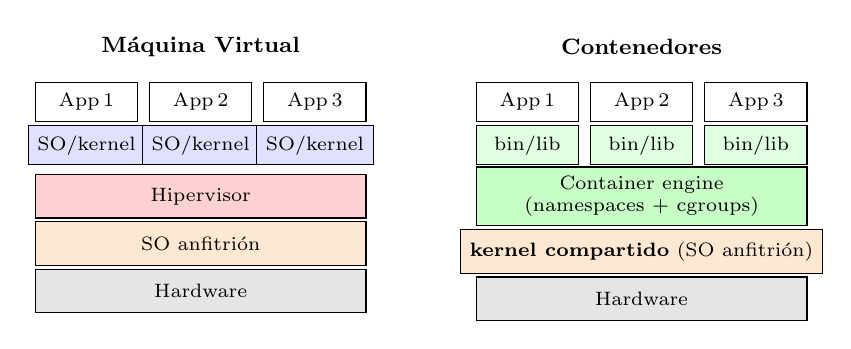
\begin{tikzpicture}[
    font=\scriptsize,
    layer/.style={draw, minimum width=4.2cm, minimum height=0.55cm, align=center},
    app/.style={draw, minimum width=1.3cm, minimum height=0.5cm, align=center},
    osb/.style={draw, fill=blue!12, minimum width=1.3cm, minimum height=0.5cm, align=center}
]
  % ===== VM (izquierda) =====
  \begin{scope}[shift={(0,0)}]
    \node[font=\footnotesize\bfseries] at (2.1,4.0) {Máquina Virtual};
    % apps + so invitado por instancia
    \foreach \x/\n in {0/1,1.45/2,2.9/3} {
      \node[app] at (\x+0.65,3.3) {App\,\n};
      \node[osb] at (\x+0.65,2.75) {SO/kernel};
    }
    \node[layer, fill=red!18] at (2.1,2.1) {Hipervisor};
    \node[layer, fill=orange!18] at (2.1,1.5) {SO anfitrión};
    \node[layer, fill=gray!20] at (2.1,0.9) {Hardware};
  \end{scope}

  % ===== Contenedores (derecha) =====
  \begin{scope}[shift={(5.6,0)}]
    \node[font=\footnotesize\bfseries] at (2.1,4.0) {Contenedores};
    \foreach \x/\n in {0/1,1.45/2,2.9/3} {
      \node[app] at (\x+0.65,3.3) {App\,\n};
      \node[app, fill=green!12] at (\x+0.65,2.75) {bin/lib};
    }
    \node[layer, fill=green!22] at (2.1,2.1) {Container engine\\(namespaces + cgroups)};
    \node[layer, fill=orange!18] at (2.1,1.4) {\textbf{kernel compartido} (SO anfitrión)};
    \node[layer, fill=gray!20] at (2.1,0.8) {Hardware};
  \end{scope}
\end{tikzpicture}
\end{center}
\diagcaption{VM: cada instancia trae su \emph{propio} SO/kernel sobre el hipervisor
(aislamiento fuerte, pesado). Contenedor: las apps comparten el \emph{mismo kernel} del
anfitrión y se separan con namespaces/cgroups (liviano, pero comparten más recursos).}

%======================================================================
\subsection{Malware}
%======================================================================

\begin{definicion}{Malware (Malicious Software)}
Cualquier programa \textbf{diseñado} para causar daño, atravesar un control o
extraer información. Lo que los distingue es haber sido concebidos
\textbf{exclusivamente con un fin malicioso}. Suelen aprovechar vulnerabilidades del
software. Un ataque usualmente usa \textbf{múltiples tipos} de malware para cada
parte del ciclo del ataque.
\end{definicion}

\subsubsection{Tipos de malware}

\begin{description}
  \item[Virus / Gusano (Worm):] su rasgo característico es la capacidad de
        \textbf{propagarse} (auto-replicarse). El virus infecta una máquina/proceso
        y usa los medios disponibles para propagarse a otras: explotando una
        vulnerabilidad remota o reescribiendo un ejecutable/recurso compartido. Un
        virus suele tener dos componentes: \textbf{replicación} + \textbf{ejecución}
        (\textit{payload}); según su payload recibe otro nombre. El \textbf{worm}
        se especializa en propagarse (su ``única misión'' es multiplicarse y ocupar
        recursos), inclusive por email; asociado a \textbf{denegación de servicio}.
        \begin{itemize}[noitemsep]
          \item Primer gusano: nació por \textbf{error} (Berkeley), se multiplicaba
                en cada máquina hasta saturar la memoria y tirar el SO.
          \item \textbf{Melissa (1999):} se propagaba por email.
          \item \textbf{SQL Slammer:} infectó $75.000$ computadoras en $10$ minutos
                explotando bases SQL de Microsoft expuestas a Internet.
        \end{itemize}
  \item[Troyano:] malware \textbf{oculto dentro de otro software} que parece
        benigno y de interés para la víctima (caballo de Troya). Sirve para
        establecer al atacante dentro del equipo. Ejemplo: \textbf{PC-Write (1986)},
        shareware de editor de texto que borraba todos los archivos. Frecuente en
        cracks de Windows/Office y en videojuegos móviles modificados.
  \item[Rootkit:] software diseñado para \textbf{ocultar} malware dentro de la
        máquina infectada. Usa ofuscación, encripción, reescritura y reemplazo de
        herramientas del sistema; toma \textbf{contramedidas activas} (p.\ ej.\
        interceptar \textit{system calls} para no aparecer en \texttt{ps} ni al
        listar directorios). Opera a nivel \textbf{kernel o usuario}; los más
        avanzados se meten en la \textbf{BIOS/bootloader} y persisten aunque se
        formatee el disco (por eso existe Secure Boot / BIOS firmada). Muy difíciles
        de detectar por antivirus.
        \begin{itemize}[noitemsep]
          \item \textbf{NTRootkit (1999):} primer rootkit para Windows NT.
          \item \textbf{Stuxnet (2010):} se escondía y propagaba por meses; solo
                actuaba al llegar a las máquinas (con firma conocida) de una planta
                nuclear de Irán (aisladas de Internet), saboteando máquinas
                industriales.
        \end{itemize}
  \item[Spyware:] software diseñado para \textbf{recolectar información} del usuario
        infectado. Se especializa en ocultar la información dentro del activo y suele
        establecer alguna forma de \textbf{covert channel (túnel)}. Algunas empresas
        lo desarrollan a pedido de gobiernos para vigilancia/espionaje (ej.\
        mencionado: Palantir).
  \item[Ransomware:] bloquea el acceso del usuario a su información (típicamente la
        \textbf{cifra}) y pide \textbf{dinero (rescate)} para restaurarla; otros
        exfiltran y piden rescate para no publicar. Apareció como uso ``creativo''
        de las criptomonedas (cobro descentralizado y difícil de rastrear).
        \begin{itemize}[noitemsep]
          \item \textbf{CryptoLocker (2013):} por mail; $\sim$U\$D 3M robados ese año.
          \item \textbf{WannaCry (2017):} explotó una vulnerabilidad conocida de
                Windows, se distribuyó por la red local; $>200$K máquinas, costo
                estimado U\$D 4B.
        \end{itemize}
  \item[Botnet:] despliega \textbf{bots/agentes multiuso} (máquinas ``zombi'') que
        quedan a la escucha de instrucciones de un \textbf{Command \& Control (C\&C)}.
        Las máquinas infectadas se usan para ataques distribuidos (DDoS), minería de
        cripto, accesos anónimos, distribuir spam, robar credenciales. La
        infraestructura C\&C es un sistema \textbf{distribuido, descentralizado, sin
        único punto de falla}. \textbf{Srizbi (2008):} la botnet más grande
        documentada, responsable de $\sim$la mitad del spam mundial ($60$B mails/día).
\end{description}

\begin{center}
\begin{tikzpicture}[
    font=\scriptsize,
    root/.style={draw, fill=red!12, rounded corners, minimum height=0.7cm, font=\footnotesize\bfseries},
    leaf/.style={draw, fill=blue!8, rounded corners, minimum width=1.7cm, minimum height=0.7cm, align=center},
    edge/.style={-{Latex}}
]
  \node[root] (mw) at (-0.75,0) {Malware};
  \node[leaf] (vir)  at (-5.0,-1.6) {Virus / Gusano\\(propaga)};
  \node[leaf] (tro)  at (-3.3,-1.6) {Troyano\\(se esconde)};
  \node[leaf] (rk)   at (-1.6,-1.6) {Rootkit\\(oculta)};
  \node[leaf] (spy)  at (0.1,-1.6)  {Spyware\\(recolecta)};
  \node[leaf] (ran)  at (1.8,-1.6)  {Ransomware\\(cifra)};
  \node[leaf] (bot)  at (3.5,-1.6)  {Botnet\\(C\&C)};
  \foreach \n in {vir,tro,rk,spy,ran,bot} \draw[edge] (mw) -- (\n.north);
\end{tikzpicture}
\end{center}
\diagcaption{Taxonomía de los tipos de malware vistos en clase. Virus/gusano y troyano
describen cómo \emph{llega/se propaga}; el resto describe el \emph{payload} o la función.}

\begin{examen}
\textbf{Definiciones que se preguntan (verdadero/falso o emparejar):}
\begin{itemize}[noitemsep]
  \item Virus/Worm $\rightarrow$ se \emph{propaga}. Troyano $\rightarrow$ se
        \emph{esconde} dentro de software benigno. Ni virus ni troyano dicen qué
        hace una vez adentro: eso es el \textbf{payload} (ransomware, C\&C, spyware\dots).
  \item Rootkit $\rightarrow$ se \emph{oculta} con contramedidas activas (no es un
        mecanismo de propagación, sino de ocultamiento/persistencia). Puede ocultar
        tanto virus como troyanos u otros programas. Se combinan: un virus se propaga,
        en cada máquina se enquista como rootkit y ejecuta un ransomware.
\end{itemize}
\end{examen}

\subsubsection{Ciclo de ataque del malware (Malware attack cycle)}

\begin{enumerate}[noitemsep]
  \item \textbf{Reconocimiento inicial (Initial Recon):} se identifica a la víctima
        y se recopila información (puntos débiles, responsables clave, redes sociales
        de empleados; se establecen relaciones falsas).
  \item \textbf{Compromiso inicial (Initial Compromise):} el malware se
        ``\textit{weaponiza}'' (se empaqueta para ser ejecutado por la víctima) y se
        compromete una o más máquinas con un ataque dirigido. Puede durar varios días.
  \item \textbf{Establecerse (Establish Foothold):} establece comunicación con su
        C\&C, asegura persistencia y almacenamiento; baja y compone nuevas
        herramientas. Suele durar minutos tras la infección inicial.
  \item \textbf{Escalar privilegios (Escalate Privileges):} eleva los privilegios
        obtenidos usando vulnerabilidades locales o remotas. Minutos.
  \item \textbf{Reconocimiento interno (Internal Recon):} mapea otras máquinas y
        usuarios de interés; prueba comunicación/visibilidad; baja nuevos malwares.
  \item \textbf{Movimiento lateral (Move Laterally):} explotación remota de
        vulnerabilidades para incrementar la base infectada.
  \item \textbf{Mantener la presencia (Maintain Presence):} persiste en las nuevas
        máquinas. (Pasos 4--7 forman un \textbf{loop}.)
  \item \textbf{Completar la misión (Complete Mission):} ejecuta su payload. Va
        exfiltrando o acumulando la información hasta enviarla en horarios de menor
        monitoreo; en ransomware, infecta la mayor cantidad posible de máquinas antes
        de activar el bloqueo.
\end{enumerate}

\begin{center}
\begin{tikzpicture}[
    font=\scriptsize,
    ph/.style={draw, fill=red!15, minimum width=1.55cm, minimum height=0.9cm, align=center},
    fl/.style={-{Latex}, thick}
]
  \node[ph] (recon) at (0,0) {Initial\\Recon};
  \node[ph] (comp)  at (1.9,0) {Initial\\Compromise};
  \node[ph] (foot)  at (3.8,0) {Establish\\Foothold};
  \node[ph] (esc)   at (5.7,0) {Escalate\\Privileges};
  \node[ph] (mission) at (8.1,0) {Complete\\Mission};

  \draw[fl] (recon) -- (comp);
  \draw[fl] (comp) -- (foot);
  \draw[fl] (foot) -- (esc);

  % loop por arriba: Internal Recon -> Move Laterally -> Maintain Presence
  \node[ph, fill=red!8] (intr) at (5.7,1.6) {Internal\\Recon};
  \node[ph, fill=red!8] (move) at (7.6,1.6) {Move\\Laterally};
  \node[ph, fill=red!8] (maint) at (4.0,1.6) {Maintain\\Presence};
  \draw[fl] (esc) -- (intr);
  \draw[fl] (intr) -- (move);
  \draw[fl] (move) to[bend left=20] (maint);
  \draw[fl] (maint) to[bend left=20] (esc.north);
  \node[font=\scriptsize, align=center] at (5.8,2.55) {loop (pasos 4--7)};

  \draw[fl] (intr) -- (mission.north);
\end{tikzpicture}
\end{center}
\diagcaption{Ciclo de ataque del malware: las primeras fases son secuenciales; escalada
de privilegios, reconocimiento interno, movimiento lateral y mantener presencia forman un
\emph{loop} que expande la base infectada antes de completar la misión (payload).}

Lo interesante: desde el reconocimiento inicial hasta el loop de escalamiento, el
ciclo es \textbf{genérico} (independiente del payload final). Por eso existen
\textbf{kits de desarrollo de malware} vendidos como producto en el mercado gris
(aunque a veces son ellos mismos troyanos, y al ser genéricos tienen más chance de
ser detectados).

\begin{ojo}
\textbf{Errores que penalizan en esta unidad:}
\begin{itemize}[noitemsep]
  \item No reconocer que una \textbf{reducción de entropía es flujo de información}
        (caso del disipador / side-channel).
  \item Afirmar que el control de acceso (matriz de acceso) evita el flujo de
        información: \textbf{no lo evita}.
  \item Usar la fórmula de flujo equivocada: condicional $H(x_s\mid y_s)$ si $y$ ya
        existía; absoluta $H(x_s)$ si $y$ se crea durante la ejecución.
\end{itemize}
\end{ojo}

\end{document}
